
\section{Personnages}
\lettrine{L}{e} c\oe{}ur des jeux de rôle réside dans la possibilité de créer, améliorer et faire évoluer son propre personnage. Voilà comment ça fonctionne dans {\jedifont Starwars reloaded}. 

\subsection{Race}
Vous pouvez choisir pour votre personnage n’importe quelle race disponible dans l'univers de Starwars. 

\subsection{Humain}
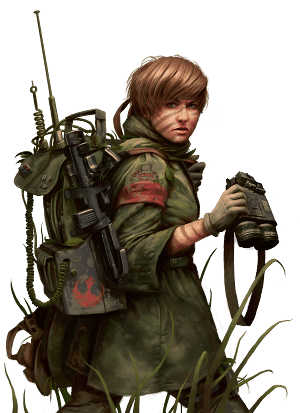
\includegraphics[width=5cm]{img/races/humain.png}
Cette race comprend aussi bien les humains au sens strict (qu’ils soient originaires de Coruscant, de Correlia, de Kuat, de Naboo...) que les humanoïdes dont les caractéristiques physiques, intellectuelles, sociales et culturelles sont suffisamment proches de celles des humains pour qu’il soit possible de les assimiler en termes de jeu. Cela inclut par exemple les iridoniens (zabraks) et les dévaroniens.

Les humains bénéficient d'un atout gratiut, cette option représente leur diversité et leur faculté d’adaptation par rapport aux autres races.

\subsection{Barabel}
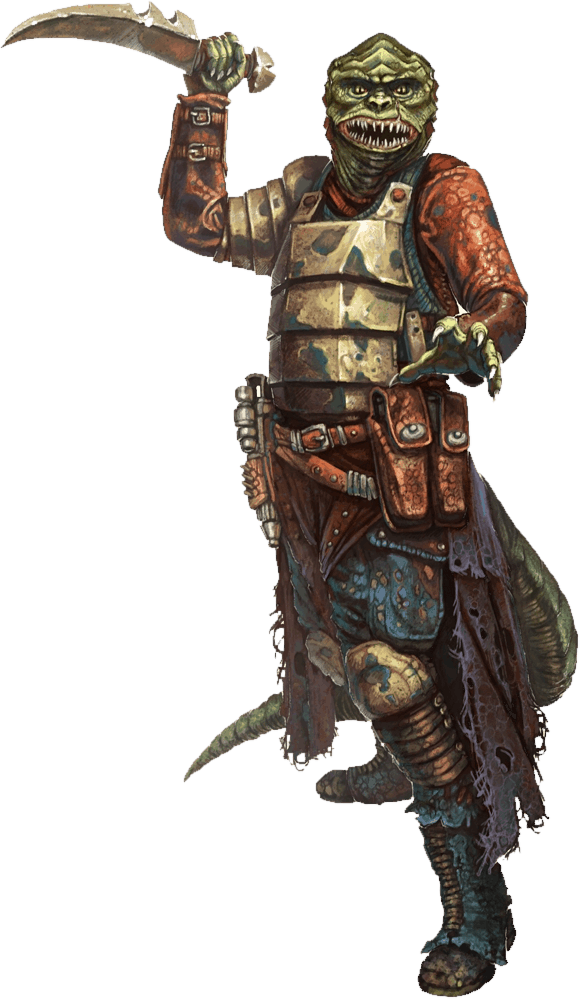
\includegraphics[width=5cm, right]{img/races/barabel.png}

Officiellement découverts l'année du couronnement de Palpatine, les indigènes primitifs de Barab I se sont rapidement intégrés à la civilisation galactique tout en demeurant paradoxalement relativement primitifs et isolés. Sur leur monde d'origine, les Barabels vivent en groupes claniques, le plus souvent matriarcaux. Ils se livrent à de nombreux conflits et tous les Barabels éprouvent une grande fascination pour la guerre, la violence, la tactique et l'armement. Les Barabels ne forment pas une race particulièrement cruelle mais il est indéniable qu'ils sont agressifs par nature, même si cela ne semble pas impliquer une volonté expansionniste (comme ce fut par exemple le cas avec les Aqualish d'Ando) et qu'ils possèdent également nombre de rituels pour commercer ou parlementer. Les indigènes de Barab ne soupçonnaient même pas l'existence d'autres mondes en raison du climat particulier de leur planète, située dangereusement près de son soleil et dont la surface ne devenait habitable que pendant la nuit, le ciel étant alors dissimulé par les nuages d'humidité en voie de condensation. 

\begin{quotebox}
	As you approach this template you get a sense that the blood and tears of many generations went into its making. A warm feeling welcomes you as you type your first words.
\end{quotebox}

\newpage % Acts as columbreak because of twocolumn option; for pagebreak use \clearpage

% For more columns, you can say \begin{dndtable}[your options here}.
% For instance, if you wanted three columns, you could say
% \begin{dndtable}{XXX}. The usual host of tabular parameters are
% aailable as well.
\header{Nice table}
\begin{dndtable}
   	\textbf{Table head}  & \textbf{Table head} \\
   	Some value  & Some value \\
   	Some value  & Some value \\
   	Some value  & Some value
\end{dndtable}

\begin{paperbox}{Do the Players need direction?}
	\lipsum[1]
\end{paperbox}

% You can optionally not include the background by saying
% begin{monsterboxnobg}
\begin{monsterbox}{Monster Foo}
	\textit{Small metasyntatic variable (golbinoid), neutral evil}\\
	\hline
	\basics[%
	armorclass = 12,
	hitpoints  = 16 (3d8 + 3),
	speed      = 50 ft
	]
	\hline
	\stats[
    STR = \stat{12}, % This stat command will autocomplete the modifier for you
    DEX = \stat{7}
	]
	\hline
	\details[%
	% If you want to use commas in these sections, enclose the
	% description in braces.
	% I'm so sorry.
	languages = {Common Lisp, Erlang},
	]
	\hline \\[1mm]
	\begin{monsteraction}[Monster-super-powers]
		This Monster has some serious superpowers!
	\end{monsteraction}
	\monstersection{Actions}
	\begin{monsteraction}[Generate text]
		This one can generate tremendous amounts of text! Though only when it wants to.
	\end{monsteraction}

	\begin{monsteraction}[More actions]
    See, here he goes again! Yet more text.
	\end{monsteraction}
\end{monsterbox}
